\documentclass[]{article}
\usepackage{amssymb,amsmath}
\usepackage{ifxetex,ifluatex}
\ifxetex
  \usepackage{fontspec,xltxtra,xunicode}
  \defaultfontfeatures{Mapping=tex-text,Scale=MatchLowercase}
\else
  \ifluatex
    \usepackage{fontspec}
    \defaultfontfeatures{Mapping=tex-text,Scale=MatchLowercase}
  \else
    \usepackage[utf8]{inputenc}
  \fi
\fi
\usepackage{color}
\usepackage{fancyvrb}
\DefineShortVerb[commandchars=\\\{\}]{\|}
\DefineVerbatimEnvironment{Highlighting}{Verbatim}{commandchars=\\\{\}}
% Add ',fontsize=\small' for more characters per line
\newenvironment{Shaded}{}{}
\newcommand{\KeywordTok}[1]{\textcolor[rgb]{0.00,0.44,0.13}{\textbf{{#1}}}}
\newcommand{\DataTypeTok}[1]{\textcolor[rgb]{0.56,0.13,0.00}{{#1}}}
\newcommand{\DecValTok}[1]{\textcolor[rgb]{0.25,0.63,0.44}{{#1}}}
\newcommand{\BaseNTok}[1]{\textcolor[rgb]{0.25,0.63,0.44}{{#1}}}
\newcommand{\FloatTok}[1]{\textcolor[rgb]{0.25,0.63,0.44}{{#1}}}
\newcommand{\CharTok}[1]{\textcolor[rgb]{0.25,0.44,0.63}{{#1}}}
\newcommand{\StringTok}[1]{\textcolor[rgb]{0.25,0.44,0.63}{{#1}}}
\newcommand{\CommentTok}[1]{\textcolor[rgb]{0.38,0.63,0.69}{\textit{{#1}}}}
\newcommand{\OtherTok}[1]{\textcolor[rgb]{0.00,0.44,0.13}{{#1}}}
\newcommand{\AlertTok}[1]{\textcolor[rgb]{1.00,0.00,0.00}{\textbf{{#1}}}}
\newcommand{\FunctionTok}[1]{\textcolor[rgb]{0.02,0.16,0.49}{{#1}}}
\newcommand{\RegionMarkerTok}[1]{{#1}}
\newcommand{\ErrorTok}[1]{\textcolor[rgb]{1.00,0.00,0.00}{\textbf{{#1}}}}
\newcommand{\NormalTok}[1]{{#1}}
% Redefine labelwidth for lists; otherwise, the enumerate package will cause
% markers to extend beyond the left margin.
\makeatletter\AtBeginDocument{%
  \renewcommand{\@listi}
    {\setlength{\labelwidth}{4em}}
}\makeatother
\usepackage{enumerate}
\usepackage{graphicx}
% We will generate all images so they have a width \maxwidth. This means
% that they will get their normal width if they fit onto the page, but
% are scaled down if they would overflow the margins.
\makeatletter
\def\maxwidth{\ifdim\Gin@nat@width>\linewidth\linewidth
\else\Gin@nat@width\fi}
\makeatother
\let\Oldincludegraphics\includegraphics
\renewcommand{\includegraphics}[1]{\Oldincludegraphics[width=8cm]{#1}}
\ifxetex
  \usepackage[setpagesize=false, % page size defined by xetex
              unicode=false, % unicode breaks when used with xetex
              xetex,
              colorlinks=true,
              linkcolor=blue]{hyperref}
\else
  \usepackage[unicode=true,
              colorlinks=true,
              linkcolor=blue]{hyperref}
\fi
\hypersetup{breaklinks=true, pdfborder={0 0 0}}
\setlength{\parindent}{0pt}
\setlength{\parskip}{6pt plus 2pt minus 1pt}
\setlength{\emergencystretch}{3em}  % prevent overfull lines
\setcounter{secnumdepth}{0}
\usepackage[margin=2cm]{geometry}

\author{
Cheshire, James\\
\texttt{james.cheshire@ucl.ac.uk}
\and
Lovelace, Robin\\
\texttt{r.lovelace@leeds.ac.uk}
}
\title{Spatial data visualisation with R}

\begin{document}
\maketitle

\section{Introduction}

\subsection{What is R?}

R is a free and open source computer program that runs on all major
operating systems. R relies primarily on the \emph{command line} for
data input: instead of interacting with the program by moving your mouse
around clicking on different parts of the screen, users enter commands
via the keyboard. This will seem to strange to people accustomed to
relying on a graphical user interface (GUI) for most of their computing,
e.g.~via popular programs such as Microsoft Excel or SPSS, yet the
approach has a number of benefits, as highlighted by Gary Sherman (2008,
p.~283), developer of the popular Geographical Informations System QGIS:

\begin{quote}
With the advent of ``modern'' GIS software, most people want to point
and click their way through life. That's good, but there is a tremendous
amount of flexibility and power waiting for you with the command line.
Many times you can do something on the command line in a fraction of the
time you can do it with a GUI.

\end{quote}
The joy of this, when you get accustomed to it, is that any command is
only ever a few keystrokes away, and the order of the commands sent to R
can be stored and repeated in scripts, saving even more time in the
long-term (more on this in section \ldots{}).

Another important attribute of R, related to its command line interface,
is that it is a fully fledged \emph{programming language}. Other GIS
programs are written in lower level languages such as C++ which are kept
at a safe distance from the users by the GUI. In R, by contrast, the
user is `close to the metal' in the sense that what he or she inputs is
the same as what R sees when it processes the request. This `openness'
can seem raw and daunting to beginners, but it is vital to R's success.
Access to R's source code and openness about how it works has enabled a
veritable army of programmers to improve R over time and add an
incredible number of extensions to its base capabilities. Consider for a
moment that there are now more than 4000 official packages for R,
allowing it to tackle almost any computational or numerical problem one
could image, and many more that one could not!

Although writing R source code and creating new packages will not appeal
to most R users, it inspires confidence to know that there is a strong
and highly skilled community of R developers. If there is a useful
spatial function that R cannot currently perform, there is a reasonable
chance that someone is working on a solution that will become available
at a later date. This constant evolution and improvement is a feature of
open source software projects not limited to R, but the range and
diversity of extensions is certainly one of its strong points. One area
where extension of R's basic capabilities has been particularly
successful is the addition of a wide variety of spatial tools.

\subsection{The rise of R's spatial capabilities}

!!! Quick history of R's spatial packages emphasizing current growth and
heavy dependence on sp.

!!!Mention exciting and recently added packages.

!!! Not sure if this is worth a complete section- we probably mention
many of the things throughout the chapter. I also wonder who really
cares!

\subsection{Why R for spatial data visualisation?}

!!! Add a bit about GIS and also the rise of information graphics-
arguably GIS has been caught out.

Aside from confusion surrounding its one character name - ``what kind of
a name is R?'' {[}1{]} and ``how can you possibly find resources for R
online?'' {[}2{]} - R may also seem a strange choice for a chapter on
\emph{spatial} data visualisation specifically. ``I thought R was just
for statistics?'' and ``Why not use a proper GIS package like ArcGIS?''
are valid questions.

The first question arises because R was traditionally conceived - and is
still primarily known - as a ``statistical programming language''
(Bivand and Gebhardt 2000). Although R does have cutting edge
statistical capabilities, this definition does not do justice to its
power and flexibility. Thus, a more accurate albeit longer definition of
R is ``an integrated suite of software facilities for data manipulation,
calculation and graphical display'' (Venables et al. 2013). It is
important to consider this wider definition before diving into R: it is
a fully fledged programming language meaning that it is highly
extensible but also that the same result can often be generated in
different ways. This can be confusing.

The second question is based on the premise that all `proper' GISs need
to operate in the same way, with primacy allocated to a mapping window
and a mouse-driven GUI interface. But when we look back at the history
of GIS and its definitions, it becomes clear that R \emph{is} fully
fledged GIS, when it is set up correctly. All early GIS programs used a
command-line interface; GUIs were only developed later as a way to run
commands without needing to remember all the command names (although
this is largely overcome by good `help' options and auto-completion). A
concise definition of a GIS is ``a computerized tool for solving
geographic problems'' (Longley et al. 2005, p.~16) and R certainly
enables this. A more expansive definition of GIS is ``a powerful set of
tools for collecting, storing, retrieving at will, transforming, and
displaying spatial data from the real world for a particular set of
purposes'' (Burrough and McDonnell, 1998, from Bivand et al. 2013,
p.~5); R excels at each of these tasks.

That being said, there are a few major differences between R and
conventional GIS programs in terms of spatial data visualisation: R is
more suited to creating one-off graphics than exploring spatial data
through repeated zooming, panning and spatial sub-setting using
custom-drawn polygons, compared with conventional GIS programs. Although
interactive maps in R can be created (e.g.~using the web interface
\texttt{shiny}), it is recommended that R is used \emph{in addition to}
rather than as a direct replacement of dedicated GIS programs,
especially now that there are myriad free options to try (Sherman 2008).
An additional point is that while dedicated GIS programs handle spatial
data by default and display the results in a single way, there are
various options in R that must be decided by the user, for example
whether to use R's base graphics or a dedicated graphics package such as
ggplot2. On the other hand, the main benefits of R for spatial data
visualisation lie in the \emph{reproducibility} of its outputs, a
feature that we will be using to great effect in this chapter.

Finally, there continues to be a clear drive towards open and
transparent datasets and this chimes well with the open access agenda
gaining momentum in academic publishing. R encourages truly transparent
and reproducable academic research by enabling anyone with an R
installation to re-run the code written to produce the results described
in a paper. This process is facilitated by the encouragement of more
consistent syntax structures and also developments in the RStudio
integrated development environment (IDE) that offers formats such as
.rmd that are executable R files in addtion to the means of sharing and
documenting code widely through Git and Subversion systems.

\subsection{R in the wild}

Examples of where R has had an important visual impact.

Might be good to mention New York Times etc here as key users of R.

\subsection{Chapter overview}

The remainder of this chapter will introduce a series of important
concepts associated with sound spatial data visualisation. It will
provide examples of R code to illustrate each concept and offer
inspiration for work with your own data.

\section{R and Spatial Data}

\subsection{Spatial Data in R}

In any data analysis project, spatial or otherwise, it is important to
have a strong understanding of the dataset before progressing. This
section will therefore begin with a description of the input data. We
will see how data can be loaded into R and exported to other formats,
before going into more detail about the underlying structure of spatial
data in R: how it `sees' spatial data is quite unique.

\subsubsection{Loading spatial data in R}

In most situations, the starting point of spatial analysis tasks is
loading in datasets. These may originate from government agencies,
remote sensing devices or `volunteered geographical information'
(Goodchild 2007). The diversity of geographical data formats is large.

R is able to import a very wide range of spatial data formats thanks to
its interface with the Geospatial Data Abstraction Library (GDAL), which
is enabled by the package \texttt{rgdal}. Below we will load data from
two spatial data formats: GPS eXchange (\texttt{.gpx}) and an ESRI
Shapefile.

\texttt{readOGR} is in fact capable of loading dozens more file formats,
so the focus is on the \emph{method} rather than the specific formats.
The `take home message' is that the \texttt{readOGR} function is capable
of loading most common spatial file formats, but behaves differently
depending on file type. Let's start with a \texttt{.gpx} file, a
tracklog recording a bicycle ride from Sheffield to Wakefield which was
uploaded Open Street Map {[}3{]}.

\begin{Shaded}
\begin{Highlighting}[]
\CommentTok{# download.file('http://www.openstreetmap.org/trace/1619756/data', destfile}
\CommentTok{# = 'data/gps-trace.gpx')}
\KeywordTok{library}\NormalTok{(rgdal)  }\CommentTok{# load the gdal package}
\NormalTok{shf2lds <- }\KeywordTok{readOGR}\NormalTok{(}\DataTypeTok{dsn =} \StringTok{"data/gps-trace.gpx"}\NormalTok{, }\DataTypeTok{layer =} \StringTok{"tracks"}\NormalTok{)  }\CommentTok{# load track}
\KeywordTok{plot}\NormalTok{(shf2lds)}
\NormalTok{shf2lds.p <- }\KeywordTok{readOGR}\NormalTok{(}\DataTypeTok{dsn =} \StringTok{"data/gps-trace.gpx"}\NormalTok{, }\DataTypeTok{layer =} \StringTok{"track_points"}\NormalTok{)  }\CommentTok{# load points}
\KeywordTok{points}\NormalTok{(shf2lds.p[}\KeywordTok{seq}\NormalTok{(}\DecValTok{1}\NormalTok{, }\DecValTok{3000}\NormalTok{, }\DecValTok{100}\NormalTok{), ])}
\end{Highlighting}
\end{Shaded}
\begin{figure}[htbp]
\centering
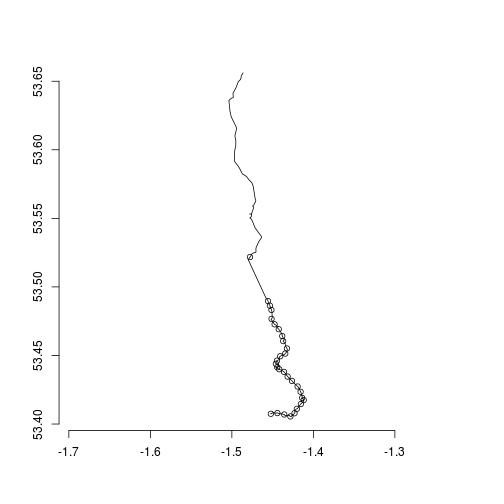
\includegraphics{figure/Leeds_to_Sheffield_GPS_data_with_latitude_and_longitude_axes.png}
\caption{Leeds to Sheffield GPS data with latitude and
longitude axes}
\end{figure}

There is a lot going on in the preceding 7 lines of code, including
functions that you are unlikely to have encountered before. Let us think
about what has happened, line-by-line.

First, we used R to \emph{download} a file from the internet, using the
function \texttt{download.file}. The two essential arguments of this
function are \texttt{url} (we could have typed \texttt{url =} before the
link) and \texttt{destfile}, the destination file. As with any function,
more optional arguments can be viewed by by typing
\texttt{?download.file}.

When \texttt{rgdal} has successfully loaded, the next task is not to
import the file directly, but to find out which \emph{layers} are
available to import, with \texttt{ogrListLayers}. The output from this
command tells us that various layers are available, including
\texttt{tracks} and \texttt{track\_points}: try it. These are imported
into R's \emph{workspace} using \texttt{readOGR}.

Finally, the basic \texttt{plot} function is used to visualize the newly
imported objects, ensuring they make sense. In the second \texttt{plot}
function, we take a subset of the object (see section \ldots{} for more
on this). To see how to add axes, enter \texttt{?axis}

As stated in the help documentation (accessed by entering
\texttt{?readOGR}), the \texttt{dsn =} argument is interpreted
differently depending on the type of file used. In the above example,
the file name was the file name. To load Shapefiles, by contrast, the
\emph{folder} containing the data is used:

\begin{Shaded}
\begin{Highlighting}[]
\NormalTok{lnd <- }\KeywordTok{readOGR}\NormalTok{(}\DataTypeTok{dsn =} \StringTok{"data/"}\NormalTok{, }\StringTok{"london_sport"}\NormalTok{)}
\end{Highlighting}
\end{Shaded}
Here, the files reside in a folder entitled \texttt{data} which in R's
current working directory (remember to check this using
\texttt{getwd()}). If the files were stored in the working directory,
one would use \texttt{dsn = "."} instead. Again, it may be wise to plot
the data that results, to ensure that it has worked correctly. Now that
the data has been loaded into R's own \texttt{sp} format, try
interrogating and plotting it, using functions such as \texttt{summary}
and \texttt{plot}.

\subsubsection{The size of spatial datasets in R}

Any data that has been read into R's \emph{workspace}, which constitutes
all objects that can be accessed by name and can be listed using the
\texttt{ls()} function, can be saved in R's own data storage file type,
\texttt{.RData}. Spatial datasets can get quite large and this can cause
problems on computers by consuming all available memory (RAM) or hard
disk space. It is wise to understand roughly how large spatial objects
are, providing insight into how long certain functions will take to run.

In the absence of prior knowledge, which of the two objects loaded in
the previous section would one expect to be larger? One could
hypothesize that the London boroughs represented by the object
\texttt{lnd} would be larger based on its greater spatial extent, but
how much larger? The answer in R is found in the function
\texttt{object.size}:

\begin{Shaded}
\begin{Highlighting}[]
\KeywordTok{object.size}\NormalTok{(shf2lds)}
\end{Highlighting}
\end{Shaded}
\begin{verbatim}
## 103168 bytes
\end{verbatim}
\begin{Shaded}
\begin{Highlighting}[]
\KeywordTok{object.size}\NormalTok{(lnd)}
\end{Highlighting}
\end{Shaded}
\begin{verbatim}
## 79168 bytes
\end{verbatim}
Surprisingly, the GPS data is larger. To see why, we can find out how
many \emph{vertices} (points connected by lines) are contained in each
dataset:

\begin{Shaded}
\begin{Highlighting}[]
\NormalTok{shf2lds.f <- }\KeywordTok{fortify}\NormalTok{(shf2lds)}
\KeywordTok{nrow}\NormalTok{(shf2lds.f)}
\end{Highlighting}
\end{Shaded}
\begin{verbatim}
## [1] 6085
\end{verbatim}
\begin{Shaded}
\begin{Highlighting}[]

\NormalTok{lnd.f <- }\KeywordTok{fortify}\NormalTok{(lnd)}
\KeywordTok{nrow}\NormalTok{(lnd.f)}
\end{Highlighting}
\end{Shaded}
\begin{verbatim}
## [1] 1102
\end{verbatim}
In the above block of code we performed two functions for each object:
1) \emph{flatten} the dataset so that each vertice is allocated a unique
row 2) use \texttt{nrow} to count the result. Note the use of the
\texttt{\textless{}-} assignment operator to create new objects with a
\texttt{.f} ending.

It is clear that the GPS data has almost 6 times the number of vertices
as does the London data, explaining its larger size. Yet when plotted,
the GPS data does not seem more detailed, implying that some of the
vertices in the object are not needed for visualisation at the scale of
the objects \emph{bounding box}.

\subsubsection{Simplifying geometries}

The wastefulness of the GPS data for visualisation (the full dataset may
be useful for other types of analysis) raises the question following
question: can the object be simplified such that its key features
features remain while substantially reducing its size? The answer is
yes. In the code below, we harness the power of the \texttt{rgeos}
package and its \texttt{gSimplify} function to simplify spatial R
objects:

\begin{Shaded}
\begin{Highlighting}[]
\KeywordTok{library}\NormalTok{(rgeos)}
\NormalTok{shf2lds.simple <- }\KeywordTok{gSimplify}\NormalTok{(shf2lds, }\DataTypeTok{tol =} \FloatTok{0.001}\NormalTok{)}
\NormalTok{(}\KeywordTok{object.size}\NormalTok{(shf2lds.simple)/}\KeywordTok{object.size}\NormalTok{(shf2lds))[}\DecValTok{1}\NormalTok{]}
\end{Highlighting}
\end{Shaded}
\begin{verbatim}
## [1] 0.03047
\end{verbatim}
\begin{Shaded}
\begin{Highlighting}[]
\KeywordTok{plot}\NormalTok{(shf2lds.simple)}
\KeywordTok{plot}\NormalTok{(shf2lds, }\DataTypeTok{col =} \StringTok{"red"}\NormalTok{, }\DataTypeTok{add =} \NormalTok{T)}
\end{Highlighting}
\end{Shaded}
In the above block of code, \texttt{gSimplify} is given the object
\texttt{shf2lds} and the \texttt{tol} argument of 0.001 (much larger
tolerance values may be needed, for data that is \emph{projected}).
Next, we divide the size of the simplified object by the original (note
the use of the \texttt{/} symbol). The output of \texttt{0.03...} tells
us that the new object is only 3\% of its original size. We can see how
this has happened by again counting the number of vertices. This time we
use the \texttt{coordinates} and \texttt{nrow} functions together:

\begin{Shaded}
\begin{Highlighting}[]
\KeywordTok{nrow}\NormalTok{(}\KeywordTok{coordinates}\NormalTok{(shf2lds.simple)[[}\DecValTok{1}\NormalTok{]][[}\DecValTok{1}\NormalTok{]])}
\end{Highlighting}
\end{Shaded}
\begin{verbatim}
## [1] 44
\end{verbatim}
The syntax of the double square brackets will seem strange, providing a
taster of how R `sees' spatial data (see section x). Do not worry about
this for now. Of interest here is that the number of vertices has
shrunk, from 6,084 to only 44, without loosing much information about
the shape of the line. To test this,try plotting the original and
simplified tracks on your computer: when visualized using the
\texttt{plot} function, object \texttt{shf2lds.simple} retains the
overall shape of the line and is virtually indistinguishable from the
original object.

This example is rather contrived because even the larger object
\texttt{shf2lds} is only 0.107 Mb, negligible compared with the
gigabytes of RAM available to modern computers. However, it underlines a
wider point: for visualizing \emph{small scale} maps, spatial data
\emph{geometries} can often be simplified to reduce processing time and
use of computer memory.

\subsubsection{Saving and exporting spatial objects}

A typical R workflow involves loading the data, processing and finally
exporting the data in a new form. \texttt{writeOGR}, the logical
counterpart of \texttt{readOGR} is ideal for this task. Imagine that we
want to view the simplified \texttt{gpx} data in software that can only
read Shapefiles. This is performed using the following command:

\begin{Shaded}
\begin{Highlighting}[]
\NormalTok{shf2lds.simple <- }\KeywordTok{SpatialLinesDataFrame}\NormalTok{(shf2lds.simple, }\KeywordTok{data.frame}\NormalTok{(}\DataTypeTok{row.names =} \StringTok{"0"}\NormalTok{, }
    \DataTypeTok{a =} \DecValTok{1}\NormalTok{))}
\KeywordTok{writeOGR}\NormalTok{(shf2lds.simple, }\DataTypeTok{layer =} \StringTok{"shf2lds"}\NormalTok{, }\DataTypeTok{dsn =} \StringTok{"data/"}\NormalTok{, }\DataTypeTok{driver =} \StringTok{"ESRI Shapefile"}\NormalTok{)}
\end{Highlighting}
\end{Shaded}
In the above code, the object was first converted into a spatial
dataframe class required by the \texttt{writeOGR} command, before being
exported as a shapefile entitled shf2lds. Unlike with \texttt{readOGR},
the driver must be specified, in this case with ``ESRI Shapefile''
{[}4{]}. The simplified GPS data is now available to other GIS programs
for further analysis. Alternatively,
\texttt{save(shf2lds.simple, file = "data/shf2lds.RData")} will save the
object in R's own spatial data format, which is described in the next
section.

\subsubsection{The structure of spatial data in R}

Spatial datasets in R are saved in their own format, defined as
\texttt{Spatial...} classes within the \texttt{sp} package. For this
reason, \texttt{sp} is the basic spatial package in R, upon which the
others depend. Spatial classes range from the basic \texttt{Spatial}
class to the complex, \texttt{SpatialPolygonsDataFrame}: the
\texttt{Spatial} class contains only two required \emph{slots}{[}5{]}:

\begin{Shaded}
\begin{Highlighting}[]
\KeywordTok{getSlots}\NormalTok{(}\StringTok{"Spatial"}\NormalTok{)}
\end{Highlighting}
\end{Shaded}
\begin{verbatim}
##        bbox proj4string 
##    "matrix"       "CRS"
\end{verbatim}
This tells us that \texttt{Spatial} objects must contain a bounding box
(\texttt{bbox}) and and CRS. Further details on these can be found by
typing \texttt{?bbox} and \texttt{?proj4string}. All other spatial
classes in R build on this foundation of a bounding box and a projection
system (which is set automatically to \texttt{NA} if it is not known).
However, more complex classes contain more slots, some of which are
lists which contain additional lists. To find out the slots of
\texttt{shf2lds.simple}, for example, we would first ascertain its class
and then use the \texttt{getSlots} command:

\begin{Shaded}
\begin{Highlighting}[]
\KeywordTok{class}\NormalTok{(shf2lds.simple)  }\CommentTok{# identify the object's class}
\end{Highlighting}
\end{Shaded}
\begin{verbatim}
## [1] "SpatialLinesDataFrame"
## attr(,"package")
## [1] "sp"
\end{verbatim}
\begin{Shaded}
\begin{Highlighting}[]
\KeywordTok{getSlots}\NormalTok{(}\StringTok{"SpatialLinesDataFrame"}\NormalTok{)  }\CommentTok{# find the associated slots}
\end{Highlighting}
\end{Shaded}
\begin{verbatim}
##         data        lines         bbox  proj4string 
## "data.frame"       "list"     "matrix"        "CRS"
\end{verbatim}
The same principles apply to all spatial classes including
\texttt{Spatial* Points}, \texttt{Polygons} \texttt{Grids} and
\texttt{Pixels} as well as associated \texttt{*DataFrame} classes. For
more information on this, see the \texttt{sp} documentation:
\texttt{?Spatial}.

\subsection{Manipulating spatial data}

\subsubsection{Coordinate reference systems}

As mentioned in the previous section, all \texttt{Spatial} objects in R
are allocated a coordinate reference system (CRS). The CRS of any
spatial object can be found using the command \texttt{proj4string}. In
some cases the CRS is not known: in this case the result will simply be
\texttt{NA}. To discover the CRS of the \texttt{lnd} object for example,
type the following:

\begin{Shaded}
\begin{Highlighting}[]
\KeywordTok{proj4string}\NormalTok{(lnd)}
\end{Highlighting}
\end{Shaded}
\begin{verbatim}
## [1] "+proj=tmerc +lat_0=49 +lon_0=-2 +k=0.9996012717 +x_0=400000 +y_0=-100000 +ellps=airy "
\end{verbatim}
The output may seem cryptic but is in fact highly informative:
\texttt{lnd} has \emph{projected} coordinates, based on the
\href{http://en.wikipedia.org/wiki/Transverse\_Mercator\_projection}{\emph{Transverse
Mercator}} system (hence \texttt{"+proj=tmerc"} in the output) and its
origin is at latitude 49N, -2E. This point is

If we \emph{know} that the CRS is incorrectly specified, it can be
re-set. In this case, for example we know that \texttt{lnd} actually has
a CRS OSGB1936. Knowing also that the code for this is 27700, it can be
updated as follows:

\begin{Shaded}
\begin{Highlighting}[]
\KeywordTok{proj4string}\NormalTok{(lnd) <- }\KeywordTok{CRS}\NormalTok{(}\StringTok{"+init=epsg:27700"}\NormalTok{)}
\end{Highlighting}
\end{Shaded}
The CRS has now been updated - note that the key details are all the
same as before. Note: this method \textbf{should never} be used as an
attempt to \emph{reproject} data from one CRS to another.

\subsubsection{Reprojecting data}

Transforming the coordinates of spatial data from one CRS to another
(reprojection) is a common task in GIS. This is because data from
national sources are generally provided in \emph{projected} coordinates
(the location on the cartesian coordinates of a map) whereas data from
GPSs and the internet are generally provided in \emph{geographic}
coordinates, with latitude and longitude measured in degrees to locate
points on the surface of the globe.

Reprojecting data in R is quite simple: all you need is a spatial object
with a known CRS and knowledge of the CRS you wish to transform it to.
To illustrate why that is necessary, try to plot the objects
\texttt{lnd} and \texttt{shf2lnd.simple} on the same map:

\begin{Shaded}
\begin{Highlighting}[]
\NormalTok{combined <- }\KeywordTok{rbind}\NormalTok{(}\KeywordTok{fortify}\NormalTok{(shf2lds.simple)[, }\DecValTok{1}\NormalTok{:}\DecValTok{2}\NormalTok{], }\KeywordTok{fortify}\NormalTok{(lnd)[, }\DecValTok{1}\NormalTok{:}\DecValTok{2}\NormalTok{])}
\KeywordTok{plot}\NormalTok{(combined)}
\end{Highlighting}
\end{Shaded}
\begin{figure}[htbp]
\centering
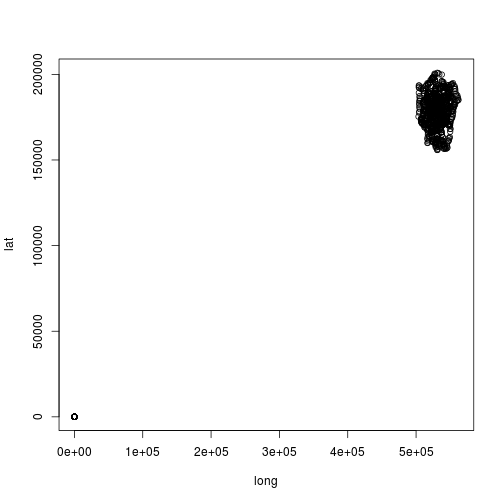
\includegraphics{figure/Plot_of_spatial_objects_with_different_CRS.png}
\caption{Plot of spatial objects with different CRS}
\end{figure}

In the above code we first extracted the coordinates of each point using
\texttt{fortify} and then plotted them using \texttt{plot}. The image
shows why reprojection is necessary: the .gpx data are on a totally
different scale than the shapefile of London. Hence the tiny dot at the
bottom right of the graph. We will now reproject the data, allowing
\texttt{lnd} and \texttt{shf2lds.simple} to be usefully plotted on the
same graphic:

\begin{Shaded}
\begin{Highlighting}[]
\NormalTok{lnd.wgs84 <- }\KeywordTok{spTransform}\NormalTok{(lnd, }\DataTypeTok{CRSobj =} \KeywordTok{CRS}\NormalTok{(}\StringTok{"+init=epsg:4326"}\NormalTok{))}
\end{Highlighting}
\end{Shaded}
The above code created a new object,\texttt{lnd.wgs84}, that contains
the same geometries as the original but in a new CRS using the
\texttt{spTransform} function. The \texttt{CRS} argument was set to
\texttt{"+init=epsg:4326"}, which represents the WGS84 CRS via an EPSG
code {[}6{]}. Now \texttt{lnd} has been reprojected we can plot it next
to the GPS data:

\begin{Shaded}
\begin{Highlighting}[]
\NormalTok{combined <- }\KeywordTok{rbind}\NormalTok{(}\KeywordTok{fortify}\NormalTok{(shf2lds.simple)[, }\DecValTok{1}\NormalTok{:}\DecValTok{2}\NormalTok{], }\KeywordTok{fortify}\NormalTok{(lnd.wgs84)[, }\DecValTok{1}\NormalTok{:}\DecValTok{2}\NormalTok{])}
\KeywordTok{plot}\NormalTok{(combined)}
\end{Highlighting}
\end{Shaded}
\begin{figure}[htbp]
\centering
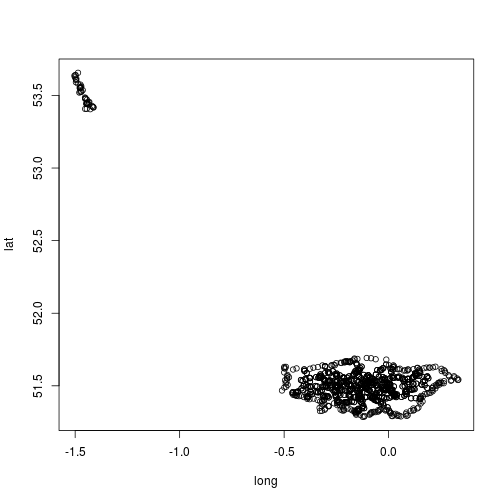
\includegraphics{figure/Plot_of_spatial_objects_sharing_the_same_CRS.png}
\caption{Plot of spatial objects sharing the same CRS}
\end{figure}

Although the plot of the reprojected data is squashed because the axis
scales are not fixed and distorted (\emph{geographic} coordinates such
as WGS84 should not usually be used for plotting), at least the relative
position and shape of both objects can now be seen. The presence of the
dotted line in the top left of the plot confirms our assumption that the
GPS data is from around Sheffield, which is northwest of London.

\subsubsection{Attribute joins}

Because boroughs are official administrative zones, there is much data
available at this level that we can link to the polygons in the
\texttt{lnd} object. We will use the example of crime data to illustrate
this data availability, which is stored in the \texttt{data} folder
available from this project's github page.

\begin{Shaded}
\begin{Highlighting}[]
\KeywordTok{load}\NormalTok{(}\StringTok{"data/crimeAg.Rdata"}\NormalTok{)  }\CommentTok{# load the crime dataset from an R dataset}
\end{Highlighting}
\end{Shaded}
After the dataset has been explored (e.g.~using the \texttt{summary} and
\texttt{head} functions) to ensure compatibility, it can be joined to
\texttt{lnd}. We will use the the \texttt{join} function in the
\texttt{plyr} package but the \texttt{merge} function could equally be
used (remember to type \texttt{library(plyr)} if needed).

\texttt{join} requires all joining variables to have the same name, but
this work has already been done {[}7{]}. Once this preparation has been
done, the join funtion is actually very simple:

\begin{Shaded}
\begin{Highlighting}[]
\NormalTok{lnd@data <- }\KeywordTok{join}\NormalTok{(lnd@data, crimeAg)}
\end{Highlighting}
\end{Shaded}
Take a look at the \texttt{lnd@data} object. You should see new
variables added, meaning the attribute join was successful.

\subsection{Spatial joins}

A spatial join, like attribute joins, is used to transfer information
from one dataset to another. There is a clearly defined direction to
spatial joins, with the \emph{target layer} receiving information from
another spatial layer based on the proximity of elements from both
layers to each other. There are three broad types of spatial join:
one-to-one, many-to-one and one-to-many. We will focus only the former
two as the third type is rarely used.

\subsubsection{One-to-one spatial joins}

One-to-one spatial joins are by far the easiest to understand and
compute because they simply involve the transfer of attributes in one
layer to another, based on location. A one-to-one join is depicted in
figure x below, and can performed using the same technique as described
in the section on spatial aggregation.

\begin{figure}[htbp]
\centering
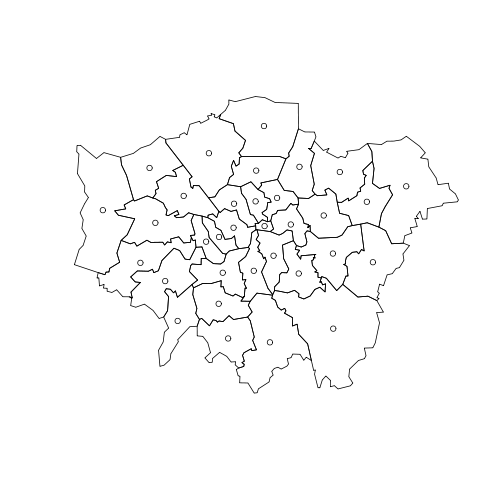
\includegraphics{figure/Illustration_of_a_one-to-one_spatial_join_.png}
\caption{Illustration of a one-to-one spatial join}
\end{figure}

\subsubsection{Many-to-one spatial joins}

Many-to-one spatial joins involve taking a spatial layer with many
elements and allocating the attributes associated with these elements to
relatively few elements in the target spatial layer. A common type of
many-to-one spatial join is the allocation of data collected at many
point sources unevenly scattered over space to polygons representing
administrative boundaries, as represented in Fig. x.

\begin{Shaded}
\begin{Highlighting}[]
\NormalTok{lnd.stations <- }\KeywordTok{readOGR}\NormalTok{(}\StringTok{"data/"}\NormalTok{, }\StringTok{"lnd-stns"}\NormalTok{, }\DataTypeTok{p4s =} \StringTok{"+init=epsg:27700"}\NormalTok{)}
\end{Highlighting}
\end{Shaded}
\begin{verbatim}
## OGR data source with driver: ESRI Shapefile 
## Source: "data/", layer: "lnd-stns"
## with 2532 features and 6 fields
## Feature type: wkbPoint with 2 dimensions
\end{verbatim}
\begin{Shaded}
\begin{Highlighting}[]
\KeywordTok{plot}\NormalTok{(lnd)}
\KeywordTok{plot}\NormalTok{(lnd.stations[}\KeywordTok{round}\NormalTok{(}\KeywordTok{runif}\NormalTok{(}\DecValTok{500}\NormalTok{, }\DecValTok{1}\NormalTok{, }\KeywordTok{nrow}\NormalTok{(lnd.stations))), ], }\DataTypeTok{add =} \NormalTok{T)}
\end{Highlighting}
\end{Shaded}
\begin{figure}[htbp]
\centering
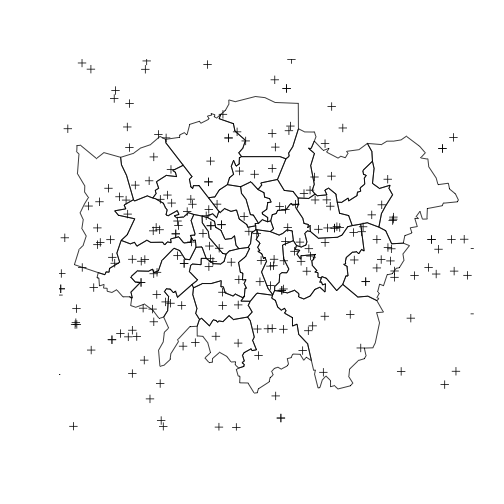
\includegraphics{figure/Input_data_for_a_spatial_join.png}
\caption{Input data for a spatial join}
\end{figure}

The above code reads in a \texttt{SpatialPointsDataFrame} consisting of
2532 transport nodes in and surrounding London and then plots a random
sample of 500 of these over the previously loaded borough level
administrative boundaries. The reason for piloting a sample of the
points rather than all of them is that the boundary data becomes
difficult to see if all of the points are piloted. It is also useful to
see and practice sampling techniques in practice; try to plot only the
first 500 points, rather than a random selection, and describe the
difference.

The most obvious issue with the point data from the perspective of a
spatial join with the borough data is that many of the points in the
dataset are in fact located outside the region of interest. Thus, the
first stage in the analysis is to filter the point data such that only
those that lie within London's administrative zones are selected. This
in itself is a kind of spatial join, and can be accomplished with the
following code.

\begin{Shaded}
\begin{Highlighting}[]
\KeywordTok{proj4string}\NormalTok{(lnd) <- }\KeywordTok{proj4string}\NormalTok{(lnd.stations)}
\NormalTok{lnd.stations <- lnd.stations[lnd, ]  }\CommentTok{# select only points within lnd}
\KeywordTok{plot}\NormalTok{(lnd.stations)  }\CommentTok{# check the result}
\end{Highlighting}
\end{Shaded}
\begin{figure}[htbp]
\centering
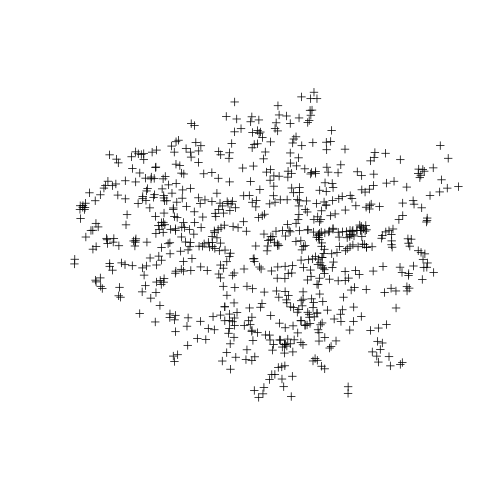
\includegraphics{figure/A_spatial_subset_of_the_points.png}
\caption{A spatial subset of the points}
\end{figure}

The station points now clearly follow the form of the \texttt{lnd}
shape, indicating that the procedure worked. Let's review the code that
allowed this to happen: the first line ensured that the CRS associated
with each layer is \emph{exactly} the same: this step should not be
required in most cases, but it is worth knowing about. Of course, if the
coordinate systems are \emph{actually} different in each layer, the
function \texttt{spTransform} will be needed to make them compatible.
This procedure is discussed in section !!!. In this case, only the name
was slightly different hence direct alteration of the CRS name via the
function \texttt{proj4string}.

The second line of code is where the magic happens and the brilliance of
R's sp package becomes clear: all that was needed was to place another
spatial object in the row index of the points (\texttt{{[}lnd, {]}}) and
R automatically understood that a subset based on location should be
produced. This line of code is an example of R's `terseness' - only a
single line of code is needed to perform what is in fact quite a complex
operation.

\subsubsection{Spatial aggregation}

Now that only stations which \emph{intersect} with the \texttt{lnd}
polygon have been selected, the next stage is to extract information
about the points within each zone. This many-to-one spatial join is also
known as \emph{spatial aggregation}. To do this there are a couple of
approaches: one using the \texttt{sp} package and the other using
\texttt{rgeos} (see Bivand et al. 2013, 5.3).

As with the \emph{spatial subest} method described above, the developers
of R have been very clever in their implementation of spatial
aggregations methods. To minimise typing and ensure consistency with R's
base functions, \texttt{sp} extends the capabilities of the
\texttt{aggregate} function to automatically detect whether the user is
asking for a spatial or a non-spatial aggregation (they are, in essence,
the same thing - we recommend learning about the non-spatial use of
\texttt{aggregate} in R for comparison).

Continuing with the example of station points in London polygons, let us
use the spatial extension of \texttt{aggregate} to count how many points
are in each borough:

\begin{Shaded}
\begin{Highlighting}[]
\NormalTok{lndStC <- }\KeywordTok{aggregate}\NormalTok{(lnd.stations, }\DataTypeTok{by =} \NormalTok{lnd, }\DataTypeTok{FUN =} \NormalTok{length)}
\KeywordTok{summary}\NormalTok{(lndStC)}
\KeywordTok{plot}\NormalTok{(lndStC)}
\end{Highlighting}
\end{Shaded}
As with the spatial subset function, the above code is extremely terse.
The aggregate function here does three things: 1) identifies which
stations are in which London borough; 2) uses this information to
perform a function on the output, in this case \texttt{length}, which
simply means ``count'' in this context; and 3) creates a new spatial
object equivalent to \texttt{lnd} but with updated attribute data to
reflect the results of the spatial aggregation. The results, with a
legend and colours added, are presented in Fig !!! below.

\begin{figure}[htbp]
\centering
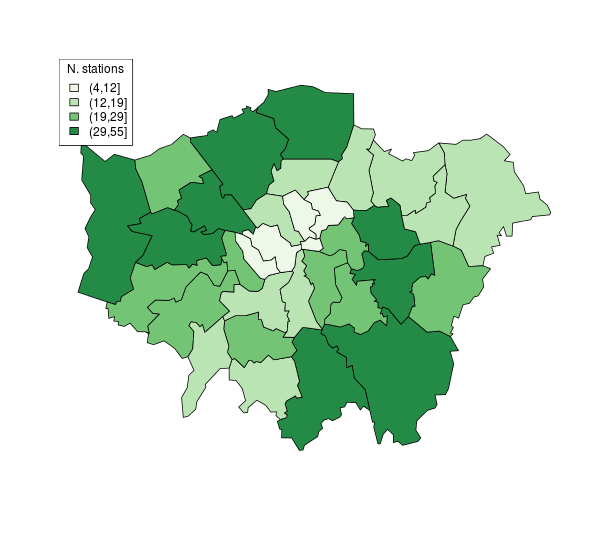
\includegraphics{figure/nStations.png}
\caption{Number of stations in London boroughs}
\end{figure}

As with any spatial attribute data stored as an \texttt{sp} object, we
can look at the attributes of the point data using the \texttt{@}
symbol:

\begin{Shaded}
\begin{Highlighting}[]
\KeywordTok{head}\NormalTok{(lnd.stations@data, }\DataTypeTok{n =} \DecValTok{2}\NormalTok{)}
\end{Highlighting}
\end{Shaded}
\begin{verbatim}
##    CODE          LEGEND FILE_NAME NUMBER                  NAME MICE
## 91 5520 Railway Station  gb_south  17607       Belmont Station   19
## 92 5520 Railway Station  gb_south  17608 Woodmansterne Station    5
\end{verbatim}
In this case we have three potentially interesting variables:
``LEGEND'', telling us what the point is, ``NAME'', and ``MICE'', which
represents the number of mice sightings reported by the public at that
point (this is a fictional variable). To illustrate the power of the
\texttt{aggregate} function, let us use it to find the average number of
mice spotted in transport points in each London borough, and the
standard deviation:

\begin{Shaded}
\begin{Highlighting}[]
\NormalTok{lndAvMice <- }\KeywordTok{aggregate}\NormalTok{(lnd.stations[}\StringTok{"MICE"}\NormalTok{], }\DataTypeTok{by =} \NormalTok{lnd, }\DataTypeTok{FUN =} \NormalTok{mean)}
\NormalTok{lndSdMice <- }\KeywordTok{aggregate}\NormalTok{(lnd.stations[}\StringTok{"MICE"}\NormalTok{], }\DataTypeTok{by =} \NormalTok{lnd, }\DataTypeTok{FUN =} \NormalTok{sd)}
\end{Highlighting}
\end{Shaded}
In the above code, \texttt{aggregate} was used to create entirely new
spatial objects that are exactly the same as \texttt{lnd}, except with
new attribute data. To add the mean mice count to the original object,
the following code can be used:

\begin{Shaded}
\begin{Highlighting}[]
\NormalTok{lnd$av.mice <- lndAvMice$MICE}
\end{Highlighting}
\end{Shaded}
The above code creates a new variable in the \texttt{lnd@data} object
entitled ``av.mice'' and populates it with desired values. Thus
\texttt{Spatial} objects can behave in the same way as data.frames when
refering to attribute variables.

\subsection{Summary}

To summarise this section, we have taken a look inside R's
representation of spatial data, learned how to manipulate these datasets
in terms of CRS transformations and attribute data and finally explored
spatial joins and aggregation. Only \emph{after} the datasets are well
understood and saved in a suitable form should we move on to
visualisation.

\section{Fundamentals of Spatial Data Visualisation}

Good maps depend on sound analysis and data preparation and can have an
enormous impact on the understanding and communication of results. It
has never been easier to produce a map. The underlying data required are
available in unprecedented volumes and the technological capabilities of
transforming them into compelling maps and graphics are increasingly
sophisticated and straightforward to use. Data and software, however,
only offer the starting points of good spatial data visualisation since
they need to be refined and calibrated by the researchers seeking to
communicate their findings. In this section we will run through the
features of a good map. We will then seek to emulate them with R in
Section XX. It is worth noting that not all good maps and graphics
contain all the features below -- they should simply be seen as
suggestions rather than firm principles.

Effective map making is hard process -- as Krygier and Wood (XXX) put it
``there is a lot to see, think about, and do'' (p6). It often comes at
the end of a period of intense data analysis and perhaps when the
priority is to get a paper finished or results published and can
therefore be rushed as a result. The beauty of R (and other scripting
languages) is the ability to save code and simply re-run it with
different data. Colours, map adornments and other parameters can
therefore be quickly applied so it is well worth creating a template
script that adheres to best practice.

We have selected ggplot2 as our package of choice for the bulk of our
maps and spatial data visualisations because it has a number of these
elements at its core. The ``gg'' in its slightly odd name stands for
``Grammar of Graphics'', which is a set of rules developed by Leland
Wilkinson (2005) in a book of the same name. Grammar in the context of
graphics works in much the same way as it does in language- it provides
a structure. The structure is informed by both human perception and also
mathematics to ensure that the resulting visualisations are both
technically sound and comprehensible. Through creating ggplot2, Hadley
Wickham, implemented these rules as well as developing ways in which
plots can be built up in layers (see Wickham, 2010). This layering
component is especially useful in the context of spatial data since it
is conceptually the same as map layers in Geographical Information
Systems (GIS).

!!!!Maps with ggplot2 !!!!Adding base maps with ggmap

First load the libraries required for this section:

\begin{Shaded}
\begin{Highlighting}[]
\KeywordTok{library}\NormalTok{(rgdal)}
\end{Highlighting}
\end{Shaded}
\begin{verbatim}
## Loading required package: sp
## rgdal: version: 0.8-10, (SVN revision 478)
## Geospatial Data Abstraction Library extensions to R successfully loaded
## Loaded GDAL runtime: GDAL 1.10.0, released 2013/04/24
## Path to GDAL shared files: /usr/share/gdal/1.10
## Loaded PROJ.4 runtime: Rel. 4.8.0, 6 March 2012, [PJ_VERSION: 480]
## Path to PROJ.4 shared files: (autodetected)
\end{verbatim}
\begin{Shaded}
\begin{Highlighting}[]
\KeywordTok{library}\NormalTok{(ggplot2)}
\KeywordTok{library}\NormalTok{(gridExtra)}
\end{Highlighting}
\end{Shaded}
\begin{verbatim}
## Loading required package: grid
\end{verbatim}
You will also need create a folder and then set it as your working
directory. Assuming your name is \texttt{Uname}, and the folder is saved
as \texttt{sdvwR} in the Desktop in Windows, use the following.

\begin{Shaded}
\begin{Highlighting}[]
\KeywordTok{setwd}\NormalTok{(}\StringTok{"c:/Users/Uname/Desktop/sdvwR"}\NormalTok{)}
\end{Highlighting}
\end{Shaded}
For this section we are going to use a map of the world to demonstrate
some of the cartographic principles discussed. A world map is available
from the Natural Earth website. The code below will download this and
save it to your working directory. It is commented out because the data
may already be on your system. Uncomment each new line (by deleting the
\texttt{\#} symbol) if you need to download and extract the data.

\begin{Shaded}
\begin{Highlighting}[]
\KeywordTok{download.file}\NormalTok{(}\DataTypeTok{url =} \StringTok{"http://www.naturalearthdata.com/http//www.naturalearthdata.com/download/110m/cultural/ne_110m_admin_0_countries.zip"}\NormalTok{, }
    \StringTok{"ne_110m_admin_0_countries.zip"}\NormalTok{, }\StringTok{"auto"}\NormalTok{)  }\CommentTok{# download file}
\KeywordTok{unzip}\NormalTok{(}\StringTok{"ne_110m_admin_0_countries.zip"}\NormalTok{, }\DataTypeTok{exdir =} \StringTok{"data/"}\NormalTok{)  }\CommentTok{# unzip to data folder}
\KeywordTok{file.remove}\NormalTok{(}\StringTok{"ne_110m_admin_0_countries.zip"}\NormalTok{)  }\CommentTok{# remove zip file}
\end{Highlighting}
\end{Shaded}
Once downloaded we can then load the data into the R console. We have
just downloaded a shapefile, which as Section XX explains, is not
handled as a ``standard'' data object in R.

\begin{Shaded}
\begin{Highlighting}[]
\NormalTok{wrld <- }\KeywordTok{readOGR}\NormalTok{(}\StringTok{"data/"}\NormalTok{, }\StringTok{"ne_110m_admin_0_countries"}\NormalTok{)}
\end{Highlighting}
\end{Shaded}
\begin{verbatim}
## OGR data source with driver: ESRI Shapefile 
## Source: "data/", layer: "ne_110m_admin_0_countries"
## with 177 features and 63 fields
## Feature type: wkbPolygon with 2 dimensions
\end{verbatim}
\begin{Shaded}
\begin{Highlighting}[]
\KeywordTok{plot}\NormalTok{(wrld)}
\end{Highlighting}
\end{Shaded}
\begin{figure}[htbp]
\centering
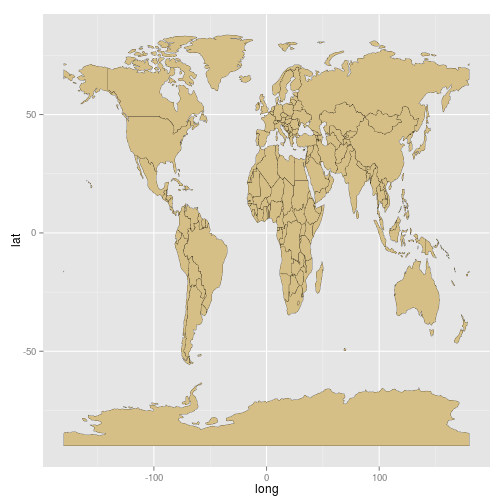
\includegraphics{figure/unnamed-chunk-4.png}
\caption{unnamed-chunk-4}
\end{figure}

To see the first ten rows of attribute information assocuiated with each
of the country boundaries type the following:

\begin{Shaded}
\begin{Highlighting}[]
\KeywordTok{head}\NormalTok{(wrld@data)[, }\DecValTok{1}\NormalTok{:}\DecValTok{5}\NormalTok{]}
\end{Highlighting}
\end{Shaded}
\begin{verbatim}
##   scalerank      featurecla labelrank           sovereignt sov_a3
## 0         1 Admin-0 country         3          Afghanistan    AFG
## 1         1 Admin-0 country         3               Angola    AGO
## 2         1 Admin-0 country         6              Albania    ALB
## 3         1 Admin-0 country         4 United Arab Emirates    ARE
## 4         1 Admin-0 country         2            Argentina    ARG
## 5         1 Admin-0 country         6              Armenia    ARM
\end{verbatim}
You can see there are a lot of columns associated with this file.
Although we will keep all of the them, we are only really interested in
the population estimate (``pop\_est'') field. Before progressing it is
is worth reprojecting the data in order that the population data can be
seen better. The coordinate reference system of the wrld shapefile is
currently WGS84. This the common latitude and longitude format that all
spatial software packages understand. From a cartographic perspective
the standard plots of this projection, of the kind produced above, are
not suitable since they distort the shapes of those countries further
from the equator. Instead the Robinson projection provides a good
compromise between areal distortion and shape preservation. We therefore
project it as follows.

\begin{Shaded}
\begin{Highlighting}[]
\NormalTok{wrld.rob <- }\KeywordTok{spTransform}\NormalTok{(wrld, }\KeywordTok{CRS}\NormalTok{(}\StringTok{"+proj=robin"}\NormalTok{))}
\KeywordTok{plot}\NormalTok{(wrld.rob)}
\end{Highlighting}
\end{Shaded}
\begin{figure}[htbp]
\centering
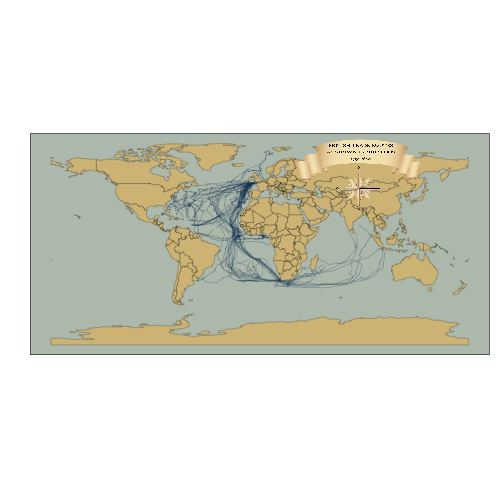
\includegraphics{figure/unnamed-chunk-6.png}
\caption{unnamed-chunk-6}
\end{figure}

``+proj=robin'' refers to the Robinson prjection. You will have spotted
from the plot that the countries in the world map are much better
proportioned.

We now need to ``fortify'' this spatial data to convert it into a format
that ggplot2 understands, we also use ``merge'' to re-attach the
attribute data that is lost in the fortify operation. !!! explain
fortify

\begin{Shaded}
\begin{Highlighting}[]
\NormalTok{wrld.rob.f <- }\KeywordTok{fortify}\NormalTok{(wrld.rob, }\DataTypeTok{region =} \StringTok{"sov_a3"}\NormalTok{)}
\end{Highlighting}
\end{Shaded}
\begin{verbatim}
## Loading required package: rgeos
## rgeos version: 0.2-19, (SVN revision 394)
##  GEOS runtime version: 3.3.8-CAPI-1.7.8 
##  Polygon checking: TRUE
\end{verbatim}
\begin{Shaded}
\begin{Highlighting}[]

\NormalTok{wrld.pop.f <- }\KeywordTok{merge}\NormalTok{(wrld.rob.f, wrld.rob@data, }\DataTypeTok{by.x =} \StringTok{"id"}\NormalTok{, }\DataTypeTok{by.y =} \StringTok{"sov_a3"}\NormalTok{)}
\end{Highlighting}
\end{Shaded}
\begin{Shaded}
\begin{Highlighting}[]
\CommentTok{# continuous colour ramp}

\NormalTok{map <- }\KeywordTok{ggplot}\NormalTok{(wrld.pop.f, }\KeywordTok{aes}\NormalTok{(long, lat, }\DataTypeTok{group =} \NormalTok{group, }\DataTypeTok{fill =} \NormalTok{pop_est)) + }\KeywordTok{geom_polygon}\NormalTok{() + }
    \KeywordTok{coord_equal}\NormalTok{() + }\KeywordTok{labs}\NormalTok{(}\DataTypeTok{x =} \StringTok{"Longitude"}\NormalTok{, }\DataTypeTok{y =} \StringTok{"Latitude"}\NormalTok{, }\DataTypeTok{fill =} \StringTok{"World Population"}\NormalTok{) + }
    \KeywordTok{ggtitle}\NormalTok{(}\StringTok{"World Population"}\NormalTok{)}

\CommentTok{# better colours with more breaks- to finish}

\NormalTok{map + }\KeywordTok{scale_fill_continuous}\NormalTok{(}\DataTypeTok{breaks =} \NormalTok{)}
\end{Highlighting}
\end{Shaded}
\begin{verbatim}
## Error: argument is missing, with no default
\end{verbatim}
\begin{Shaded}
\begin{Highlighting}[]

\CommentTok{# categorical variables}
\end{Highlighting}
\end{Shaded}
\section{Conforming to colour conventions}

Colour has an enormous impact on how people will percieve your graphic.
``Readers'' of a map come to it with a range of pre-conceptions about
how the world looks. If the map's purpose is to clearly communicate data
then it is often advisable to conform to conventions so as not to
disorientate readers to ensure they can focus on the key messages
contained in the data. A good example of this is the use of blue for
bodies of water and green for landmass. The code example below generates
two plots with our wrld.pop.f object. The first colours the land blue
and the sea (in this case the background to the map) green and the
second is more conventional. We use the ``grid.arrange'' function from
the ``gridExtra'' package to display the maps side by side.

\begin{Shaded}
\begin{Highlighting}[]
\NormalTok{map2 <- }\KeywordTok{ggplot}\NormalTok{(wrld.pop.f, }\KeywordTok{aes}\NormalTok{(long, lat, }\DataTypeTok{group =} \NormalTok{group)) + }\KeywordTok{coord_equal}\NormalTok{()}

\NormalTok{blue <- map2 + }\KeywordTok{geom_polygon}\NormalTok{(}\DataTypeTok{fill =} \StringTok{"light blue"}\NormalTok{) + }\KeywordTok{theme}\NormalTok{(}\DataTypeTok{panel.background =} \KeywordTok{element_rect}\NormalTok{(}\DataTypeTok{fill =} \StringTok{"dark green"}\NormalTok{))}

\NormalTok{green <- map2 + }\KeywordTok{geom_polygon}\NormalTok{(}\DataTypeTok{fill =} \StringTok{"dark green"}\NormalTok{) + }\KeywordTok{theme}\NormalTok{(}\DataTypeTok{panel.background =} \KeywordTok{element_rect}\NormalTok{(}\DataTypeTok{fill =} \StringTok{"light blue"}\NormalTok{))}

\KeywordTok{grid.arrange}\NormalTok{(blue, green, }\DataTypeTok{ncol =} \DecValTok{2}\NormalTok{)}
\end{Highlighting}
\end{Shaded}
\begin{figure}[htbp]
\centering
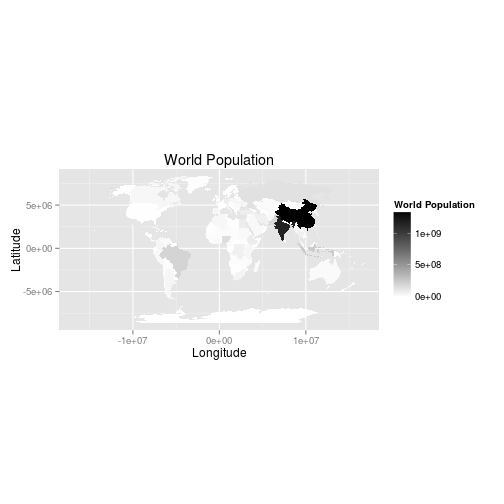
\includegraphics{figure/unnamed-chunk-9.png}
\caption{unnamed-chunk-9}
\end{figure}

\section{Experimenting with line colour and line widths}

In addition to conforming to colour conventions, line colour and width
offer important parameters, which are often overlooked tools for
increasing the legibility of a graphic. As the code below demonstrates,
it is possible to adjust line colour through using the ``colour''
parameter and the line width using the ``lwd'' parameter. The impact of
different line widths will vary depending on your screen size and
resolution. If you save the plot to pdf (or an image) then the size at
which you do this will also affect the line widths.

\begin{Shaded}
\begin{Highlighting}[]
\NormalTok{map3 <- map2 + }\KeywordTok{theme}\NormalTok{(}\DataTypeTok{panel.background =} \KeywordTok{element_rect}\NormalTok{(}\DataTypeTok{fill =} \StringTok{"light blue"}\NormalTok{))}

\NormalTok{yellow <- map3 + }\KeywordTok{geom_polygon}\NormalTok{(}\DataTypeTok{fill =} \StringTok{"dark green"}\NormalTok{, }\DataTypeTok{colour =} \StringTok{"yellow"}\NormalTok{)}

\NormalTok{black <- map3 + }\KeywordTok{geom_polygon}\NormalTok{(}\DataTypeTok{fill =} \StringTok{"dark green"}\NormalTok{, }\DataTypeTok{colour =} \StringTok{"black"}\NormalTok{)}

\NormalTok{thin <- map3 + }\KeywordTok{geom_polygon}\NormalTok{(}\DataTypeTok{fill =} \StringTok{"dark green"}\NormalTok{, }\DataTypeTok{colour =} \StringTok{"black"}\NormalTok{, }\DataTypeTok{lwd =} \FloatTok{0.1}\NormalTok{)}

\NormalTok{thick <- map3 + }\KeywordTok{geom_polygon}\NormalTok{(}\DataTypeTok{fill =} \StringTok{"dark green"}\NormalTok{, }\DataTypeTok{colour =} \StringTok{"black"}\NormalTok{, }\DataTypeTok{lwd =} \FloatTok{1.5}\NormalTok{)}

\KeywordTok{grid.arrange}\NormalTok{(yellow, black, thick, thin, }\DataTypeTok{ncol =} \DecValTok{2}\NormalTok{)}
\end{Highlighting}
\end{Shaded}
\begin{figure}[htbp]
\centering
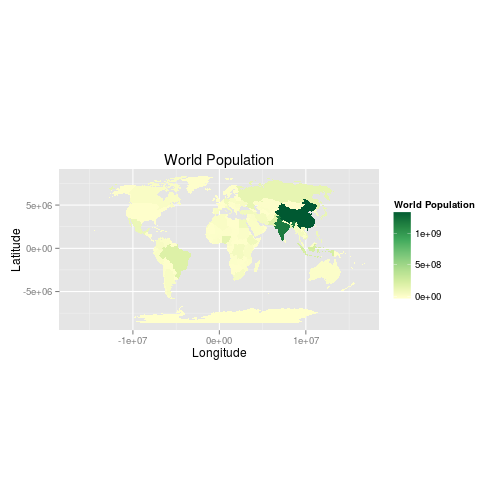
\includegraphics{figure/unnamed-chunk-10.png}
\caption{unnamed-chunk-10}
\end{figure}

There are other parameters such as layer transparency that can be
applied to all aspects of the plot - both points, lines and polygons -
that we will reference in later examples in this chapter.

\section{Map Adornments and Annotations}

Map adornments and annotations are essential to orientate the viewer and
provide context; they include graticules, north arrows, scale bars and
data attribution. Not all are required on a single map, indeed it is
often best that they are used sparingly to avoid unecessary clutter
(Monkhouse and Wilkinson, 1971). Unfortunately it is not always as
straightforward to add these in R, and perhaps less so using the ggplot2
paradigm, when compared to a conventional GIS. Here we will outline the
ways in which annotations can be added.

!!!! In the maps created so far, we have defined the \emph{aesthetics}
of the map in the foundation function \texttt{ggplot}. The result of
this is that all subsequent layers are expected to have the same
variables and essentially contain data with the same dimensions as
original dataset. But what if we want to add a new layer from a
completely different dataset To do this, we must not add any arguments
to the \texttt{ggplot} function, only adding data sources one layer at a
time:

\section{North arrow}

In the maps created so far, we have defined the \emph{aesthetics} of the
map in the foundation function \texttt{ggplot}. The result of this is
that all subsequent layers are expected to have the same variables and
essentially contain data with the same dimensions as original dataset.
But what if we want to add a new layer from a completely different
dataset, e.g.~to add an arrow? To do this, we must not add any arguments
to the \texttt{ggplot} function, only adding data sources one layer at a
time:

Here we create an empty plot, meaning that each new layer must be given
its own dataset. While more code is needed in this example, it enables
much greater flexibility with regards to what can be included in new
layer contents. Another possibility is to use the \texttt{segment} geom
to add a pre-made arrow: !!! This needs to sorted - doesn't compile
Robin

\begin{Shaded}
\begin{Highlighting}[]
\KeywordTok{ggplot}\NormalTok{() + }\KeywordTok{geom_polygon}\NormalTok{(}\DataTypeTok{data =} \NormalTok{wrld.pop.f, }\KeywordTok{aes}\NormalTok{(long, lat, }\DataTypeTok{group =} \NormalTok{group, }\DataTypeTok{fill =} \NormalTok{pop_est)) + }
    \KeywordTok{geom_line}\NormalTok{(}\KeywordTok{aes}\NormalTok{(}\DataTypeTok{x =} \KeywordTok{c}\NormalTok{(-}\DecValTok{160}\NormalTok{, -}\DecValTok{160}\NormalTok{), }\DataTypeTok{y =} \KeywordTok{c}\NormalTok{(}\DecValTok{0}\NormalTok{, }\DecValTok{25}\NormalTok{)), }\DataTypeTok{arrow =} \KeywordTok{arrow}\NormalTok{())}
\end{Highlighting}
\end{Shaded}
\begin{figure}[htbp]
\centering
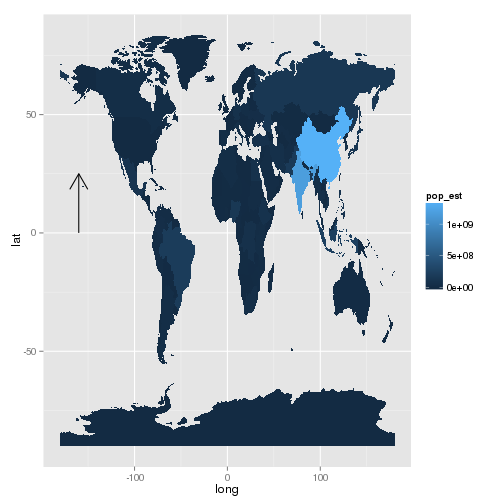
\includegraphics{figure/World_map_with_a_North_arrow.png}
\caption{World map with a North arrow}
\end{figure}

\section{Scale bar}

!!! use geom\_segment with geom\_text

There is an almost infinite number of different combinations of the
above parameters so take inspiration from maps and graphics you have
seen and liked. The process is an iterative one, it will take multiple
attempts to get right. Show your map to friends and colleagues- all will
have an opinion but don't be afraid to stand by the decisions you have
taken.

!!!Consistency- across papers.

ggmap is a package that uses the ggplot2 syntax as a template to create
maps with image tiles from the likes of Google and OpenStreetMap:

\section{Adding Basemaps To Your Plots}

\begin{Shaded}
\begin{Highlighting}[]
\KeywordTok{library}\NormalTok{(ggmap)}
\end{Highlighting}
\end{Shaded}
!!! adapt to the lnd.stations object.

The sport object is in British National Grid but the ggmap image tiles
are in WGS84. We therefore need to use the sport.wgs84 object created in
the reprojection operation earlier.

The first job is to calculate the bounding box (bb for short) of the
sport.wgs84 object to identify the geographic extent of the image tiles
that we need.

\begin{Shaded}
\begin{Highlighting}[]
\NormalTok{b <- }\KeywordTok{bbox}\NormalTok{(sport.wgs84)}
\end{Highlighting}
\end{Shaded}
\begin{verbatim}
## Error: error in evaluating the argument 'obj' in selecting a method for function 'bbox': Error: object 'sport.wgs84' not found
\end{verbatim}
\begin{Shaded}
\begin{Highlighting}[]
\NormalTok{b[}\DecValTok{1}\NormalTok{, ] <- (b[}\DecValTok{1}\NormalTok{, ] - }\KeywordTok{mean}\NormalTok{(b[}\DecValTok{1}\NormalTok{, ])) * }\FloatTok{1.05} \NormalTok{+ }\KeywordTok{mean}\NormalTok{(b[}\DecValTok{1}\NormalTok{, ])}
\end{Highlighting}
\end{Shaded}
\begin{verbatim}
## Error: object 'b' not found
\end{verbatim}
\begin{Shaded}
\begin{Highlighting}[]
\NormalTok{b[}\DecValTok{2}\NormalTok{, ] <- (b[}\DecValTok{2}\NormalTok{, ] - }\KeywordTok{mean}\NormalTok{(b[}\DecValTok{2}\NormalTok{, ])) * }\FloatTok{1.05} \NormalTok{+ }\KeywordTok{mean}\NormalTok{(b[}\DecValTok{2}\NormalTok{, ])}
\end{Highlighting}
\end{Shaded}
\begin{verbatim}
## Error: object 'b' not found
\end{verbatim}
\begin{Shaded}
\begin{Highlighting}[]
\CommentTok{# scale longitude and latitude (increase bb by 5% for plot) replace 1.05}
\CommentTok{# with 1.xx for an xx% increase in the plot size}
\end{Highlighting}
\end{Shaded}
This is then fed into the \texttt{get\_map} function as the location
parameter. The syntax below contains 2 functions. \texttt{ggmap} is
required to produce the plot and provides the base map data.

\begin{Shaded}
\begin{Highlighting}[]
\NormalTok{lnd.b1 <- }\KeywordTok{ggmap}\NormalTok{(}\KeywordTok{get_map}\NormalTok{(}\DataTypeTok{location =} \NormalTok{b))}
\end{Highlighting}
\end{Shaded}
\begin{verbatim}
## Error: object 'b' not found
\end{verbatim}
In much the same way as we did above we can then layer the plot with
different geoms.

First fortify the sport.wgs84 object and then merge with the required
attribute data (we already did this step to create the sport.f object).

\begin{Shaded}
\begin{Highlighting}[]
\NormalTok{sport.wgs84.f <- }\KeywordTok{fortify}\NormalTok{(sport.wgs84, }\DataTypeTok{region =} \StringTok{"ons_label"}\NormalTok{)}
\end{Highlighting}
\end{Shaded}
\begin{verbatim}
## Error: object 'sport.wgs84' not found
\end{verbatim}
\begin{Shaded}
\begin{Highlighting}[]
\NormalTok{sport.wgs84.f <- }\KeywordTok{merge}\NormalTok{(sport.wgs84.f, sport.wgs84@data, }\DataTypeTok{by.x =} \StringTok{"id"}\NormalTok{, }\DataTypeTok{by.y =} \StringTok{"ons_label"}\NormalTok{)}
\end{Highlighting}
\end{Shaded}
\begin{verbatim}
## Error: object 'sport.wgs84.f' not found
\end{verbatim}
We can now overlay this on our base map.

\begin{Shaded}
\begin{Highlighting}[]
\NormalTok{lnd.b1 + }\KeywordTok{geom_polygon}\NormalTok{(}\DataTypeTok{data =} \NormalTok{sport.wgs84.f, }\KeywordTok{aes}\NormalTok{(}\DataTypeTok{x =} \NormalTok{long, }\DataTypeTok{y =} \NormalTok{lat, }\DataTypeTok{group =} \NormalTok{group, }
    \DataTypeTok{fill =} \NormalTok{Partic_Per), }\DataTypeTok{alpha =} \FloatTok{0.5}\NormalTok{)}
\end{Highlighting}
\end{Shaded}
The code above contains a lot of parameters. Use the ggplot2 help pages
to find out what they are. The resulting map looks okay, but it would be
improved with a simpler base map in black and white. A design firm
called stamen provide the tiles we need and they can be brought into the
plot with the \texttt{get\_map} function:

\begin{Shaded}
\begin{Highlighting}[]
\NormalTok{lnd.b2 <- }\KeywordTok{ggmap}\NormalTok{(}\KeywordTok{get_map}\NormalTok{(}\DataTypeTok{location =} \NormalTok{b, }\DataTypeTok{source =} \StringTok{"stamen"}\NormalTok{, }\DataTypeTok{maptype =} \StringTok{"toner"}\NormalTok{, }
    \DataTypeTok{crop =} \NormalTok{T))}
\end{Highlighting}
\end{Shaded}
\begin{verbatim}
## Error: object 'b' not found
\end{verbatim}
We can then produce the plot as before.

\begin{Shaded}
\begin{Highlighting}[]
\NormalTok{lnd.b2 + }\KeywordTok{geom_polygon}\NormalTok{(}\DataTypeTok{data =} \NormalTok{sport.wgs84.f, }\KeywordTok{aes}\NormalTok{(}\DataTypeTok{x =} \NormalTok{long, }\DataTypeTok{y =} \NormalTok{lat, }\DataTypeTok{group =} \NormalTok{group, }
    \DataTypeTok{fill =} \NormalTok{Partic_Per), }\DataTypeTok{alpha =} \FloatTok{0.5}\NormalTok{)}
\end{Highlighting}
\end{Shaded}
Finally, if we want to increase the detail of the base map, get\_map has
a zoom parameter.

\begin{Shaded}
\begin{Highlighting}[]
\NormalTok{lnd.b3 <- }\KeywordTok{ggmap}\NormalTok{(}\KeywordTok{get_map}\NormalTok{(}\DataTypeTok{location =} \NormalTok{b, }\DataTypeTok{source =} \StringTok{"stamen"}\NormalTok{, }\DataTypeTok{maptype =} \StringTok{"toner"}\NormalTok{, }
    \DataTypeTok{crop =} \NormalTok{T, }\DataTypeTok{zoom =} \DecValTok{11}\NormalTok{))}
\end{Highlighting}
\end{Shaded}
\begin{verbatim}
## Error: object 'b' not found
\end{verbatim}
\begin{Shaded}
\begin{Highlighting}[]

\NormalTok{lnd.b3 + }\KeywordTok{geom_polygon}\NormalTok{(}\DataTypeTok{data =} \NormalTok{sport.wgs84.f, }\KeywordTok{aes}\NormalTok{(}\DataTypeTok{x =} \NormalTok{long, }\DataTypeTok{y =} \NormalTok{lat, }\DataTypeTok{group =} \NormalTok{group, }
    \DataTypeTok{fill =} \NormalTok{Partic_Per), }\DataTypeTok{alpha =} \FloatTok{0.5}\NormalTok{)}
\end{Highlighting}
\end{Shaded}
\begin{verbatim}
## Error: object 'lnd.b3' not found
\end{verbatim}
\section{A Final Example}

Here we present a final example that draws upon the many advanced
concepts discussed in this chapter to produce a map of 18th Century
Shipping flows.

\begin{Shaded}
\begin{Highlighting}[]
\KeywordTok{library}\NormalTok{(ggplot2)}
\KeywordTok{library}\NormalTok{(png)}
\NormalTok{wrld <- }\KeywordTok{readOGR}\NormalTok{(}\StringTok{"."}\NormalTok{, }\StringTok{"ne_110m_admin_0_countries"}\NormalTok{)}
\end{Highlighting}
\end{Shaded}
\begin{verbatim}
## Error: Cannot open file
\end{verbatim}
\begin{Shaded}
\begin{Highlighting}[]
\NormalTok{btitle <- }\KeywordTok{readPNG}\NormalTok{(}\StringTok{"figure/brit_titles.png"}\NormalTok{)}
\NormalTok{compass <- }\KeywordTok{readPNG}\NormalTok{(}\StringTok{"figure/windrose.png"}\NormalTok{)}
\NormalTok{earth <- }\KeywordTok{readPNG}\NormalTok{(}\StringTok{"figure/earth_raster.png"}\NormalTok{)}
\NormalTok{bdata <- }\KeywordTok{read.csv}\NormalTok{(}\StringTok{"data/british_shipping_example.csv"}\NormalTok{)}
\end{Highlighting}
\end{Shaded}
\begin{Shaded}
\begin{Highlighting}[]
\NormalTok{xquiet <- }\KeywordTok{scale_x_continuous}\NormalTok{(}\StringTok{""}\NormalTok{, }\DataTypeTok{breaks =} \OtherTok{NULL}\NormalTok{)}
\NormalTok{yquiet <- }\KeywordTok{scale_y_continuous}\NormalTok{(}\StringTok{""}\NormalTok{, }\DataTypeTok{breaks =} \OtherTok{NULL}\NormalTok{)}
\NormalTok{quiet <- }\KeywordTok{list}\NormalTok{(xquiet, yquiet)}
\end{Highlighting}
\end{Shaded}
\begin{Shaded}
\begin{Highlighting}[]
\NormalTok{wrld.pop.f <- }\KeywordTok{fortify}\NormalTok{(wrld, }\DataTypeTok{region =} \StringTok{"sov_a3"}\NormalTok{)}
\end{Highlighting}
\end{Shaded}
\begin{verbatim}
## Error: object 'wrld' not found
\end{verbatim}
\begin{Shaded}
\begin{Highlighting}[]
\NormalTok{base <- }\KeywordTok{ggplot}\NormalTok{(wrld.pop.f, }\KeywordTok{aes}\NormalTok{(}\DataTypeTok{x =} \NormalTok{long, }\DataTypeTok{y =} \NormalTok{lat))}
\end{Highlighting}
\end{Shaded}
\begin{verbatim}
## Error: object 'wrld.pop.f' not found
\end{verbatim}
\begin{Shaded}
\begin{Highlighting}[]
\NormalTok{route <- }\KeywordTok{c}\NormalTok{(}\KeywordTok{geom_path}\NormalTok{(}\KeywordTok{aes}\NormalTok{(long, lat, }\DataTypeTok{group =} \KeywordTok{paste}\NormalTok{(bdata$trp, bdata$group.regroup, }
    \DataTypeTok{sep =} \StringTok{"."}\NormalTok{)), }\DataTypeTok{colour =} \StringTok{"#0F3B5F"}\NormalTok{, }\DataTypeTok{size =} \FloatTok{0.2}\NormalTok{, }\DataTypeTok{data =} \NormalTok{bdata, }\DataTypeTok{alpha =} \FloatTok{0.5}\NormalTok{, }
    \DataTypeTok{lineend =} \StringTok{"round"}\NormalTok{))}
\end{Highlighting}
\end{Shaded}
\begin{Shaded}
\begin{Highlighting}[]
\NormalTok{wrld <- }\KeywordTok{c}\NormalTok{(}\KeywordTok{geom_polygon}\NormalTok{(}\KeywordTok{aes}\NormalTok{(}\DataTypeTok{group =} \NormalTok{group), }\DataTypeTok{size =} \FloatTok{0.1}\NormalTok{, }\DataTypeTok{colour =} \StringTok{"black"}\NormalTok{, }\DataTypeTok{fill =} \StringTok{"#D6BF86"}\NormalTok{, }
    \DataTypeTok{data =} \NormalTok{wrld.pop.f, }\DataTypeTok{alpha =} \DecValTok{1}\NormalTok{))}
\end{Highlighting}
\end{Shaded}
\begin{verbatim}
## Error: object 'wrld.pop.f' not found
\end{verbatim}
\begin{Shaded}
\begin{Highlighting}[]
\NormalTok{base + route + wrld + }\KeywordTok{theme}\NormalTok{(}\DataTypeTok{panel.background =} \KeywordTok{element_rect}\NormalTok{(}\DataTypeTok{fill =} \StringTok{"#BAC4B9"}\NormalTok{, }
    \DataTypeTok{colour =} \StringTok{"black"}\NormalTok{)) + }\KeywordTok{annotation_raster}\NormalTok{(btitle, }\DataTypeTok{xmin =} \DecValTok{30}\NormalTok{, }\DataTypeTok{xmax =} \DecValTok{140}\NormalTok{, }\DataTypeTok{ymin =} \DecValTok{51}\NormalTok{, }
    \DataTypeTok{ymax =} \DecValTok{87}\NormalTok{) + }\KeywordTok{annotation_raster}\NormalTok{(compass, }\DataTypeTok{xmin =} \DecValTok{65}\NormalTok{, }\DataTypeTok{xmax =} \DecValTok{105}\NormalTok{, }\DataTypeTok{ymin =} \DecValTok{25}\NormalTok{, }
    \DataTypeTok{ymax =} \DecValTok{65}\NormalTok{) + }\KeywordTok{coord_equal}\NormalTok{() + quiet}
\end{Highlighting}
\end{Shaded}
\begin{verbatim}
## Error: object 'base' not found
\end{verbatim}
\begin{Shaded}
\begin{Highlighting}[]
\NormalTok{base + }\KeywordTok{annotation_raster}\NormalTok{(earth, }\DataTypeTok{xmin =} \NormalTok{-}\DecValTok{180}\NormalTok{, }\DataTypeTok{xmax =} \DecValTok{180}\NormalTok{, }\DataTypeTok{ymin =} \NormalTok{-}\DecValTok{90}\NormalTok{, }\DataTypeTok{ymax =} \DecValTok{90}\NormalTok{) + }
    \NormalTok{route + }\KeywordTok{theme}\NormalTok{(}\DataTypeTok{panel.background =} \KeywordTok{element_rect}\NormalTok{(}\DataTypeTok{fill =} \StringTok{"#BAC4B9"}\NormalTok{, }\DataTypeTok{colour =} \StringTok{"black"}\NormalTok{)) + }
    \KeywordTok{annotation_raster}\NormalTok{(btitle, }\DataTypeTok{xmin =} \DecValTok{30}\NormalTok{, }\DataTypeTok{xmax =} \DecValTok{140}\NormalTok{, }\DataTypeTok{ymin =} \DecValTok{51}\NormalTok{, }\DataTypeTok{ymax =} \DecValTok{87}\NormalTok{) + }
    \KeywordTok{annotation_raster}\NormalTok{(compass, }\DataTypeTok{xmin =} \DecValTok{65}\NormalTok{, }\DataTypeTok{xmax =} \DecValTok{105}\NormalTok{, }\DataTypeTok{ymin =} \DecValTok{25}\NormalTok{, }\DataTypeTok{ymax =} \DecValTok{65}\NormalTok{) + }
    \KeywordTok{coord_equal}\NormalTok{() + quiet}
\end{Highlighting}
\end{Shaded}
\begin{verbatim}
## Error: object 'base' not found
\end{verbatim}
!!!change the colour of the routes to make them stand out more.

\section{Recap and Conclusions}

\newpage \section{References}

Bivand, R., \& Gebhardt, A. (2000). Implementing functions for spatial
statistical analysis using the language. Journal of Geographical
Systems, 2(3), 307--317.

Bivand, R. S., Pebesma, E. J., \& Rubio, V. G. (2008). Applied spatial
data: analysis with R. Springer.

Burrough, P. A. \& McDonnell, R. A. (1998). Principals of Geographic
Information Systems (revised edition). Clarendon Press, Oxford.

Goodchild, M. F. (2007). Citizens as sensors: the world of volunteered
geography. GeoJournal, 69(4), 211--221.

Harris, R. (2012). A Short Introduction to R.
\href{http://www.social-statistics.org/}{social-statistics.org}.

Kabacoff, R. (2011). R in Action. Manning Publications Co.

Krygier, J. Wood, D. 2011. Making Maps: A Visual Guide to Map Design for
GIS (2nd Ed.). New York: The Guildford Press.

Longley, P., Goodchild, M. F., Maguire, D. J., \& Rhind, D. W. (2005).
Geographic information systems and science. John Wiley \& Sons.

Monkhouse, F.J. and Wilkinson, H. R. 1973. Maps and Diagrams Their
Compilation and Construction (3rd Edition, reprinted with revisions).
London: Methuen \& Co Ltd.

Ramsey, P., \& Dubovsky, D. (2013). Geospatial Software's Open Future.
GeoInformatics, 16(4).

Sherman, G. (2008). Desktop GIS: Mapping the Planet with Open Source
Tools. Pragmatic Bookshelf.

Torfs and Brauer (2012). A (very) short Introduction to R. The
Comprehensive R Archive Network.

Venables, W. N., Smith, D. M., \& Team, R. D. C. (2013). An introduction
to R. The Comprehensive R Archive Network (CRAN). Retrieved from
http://cran.ma.imperial.ac.uk/doc/manuals/r-devel/R-intro.pdf .

Wickham, H. (2009). ggplot2: elegant graphics for data analysis.
Springer.

Wickham, H. 2010. A Layered Grammar of Graphics. American Statistical
Association, Institute of Mathematics Statistics and Interface
Foundation of North America Journal of Computational and Graphical
Statistics. 19, 1: 3-28

\section{Endnotes}

\begin{enumerate}[1.]
\item
  R's name originates from the creators of R, Ross Ihaka and Robert
  Gentleman. R is an open source implementation of the statistical
  programming language S, so its name is also a play on words that makes
  implicit reference to this.
\item
  R is notoriously difficult to search for on major search engines, as
  it is such a common letter with many other uses beyond the name of a
  statistical programming language. This should not be a deterrent, as R
  has a wealth of excellent online resources. To overcome the issue, you
  can either be more specific with the search term (e.g. ``R spatial
  statistics'') or use an R specific search engine such as
  \href{http://www.rseek.org/}{rseek.org}. You can also search of online
  help \emph{from within R} using the command \texttt{RSiteSearch}. E.g.
  \texttt{RSiteSearch("spatial statistics")}. Experiment and see which
  you prefer!
\item
  For more information about this ride, please see
  \href{http://robinlovelace.net/ecotech/2013/10/13/bicycle-trailer-move.html}{robinlovelace.net}.
\item
  A complete list of drivers for importing and exporting spatial data
  can be displayed by typing \texttt{getGDALDriverNames()}.
\item
  Slots are elements found `inside' classes of the
  \href{http://adv-r.had.co.nz/S4.html}{S4 object system}. While the
  sub-elements of S3 objects such as \texttt{data.frame} are referred to
  using the \texttt{\$} symbol, the slots of S4 objects are identified
  using \texttt{@}. Thus, the variable \texttt{x} of dataframe
  \texttt{df} can be referred to with \texttt{df\$x}. In the same way,
  the data associated with a polygon layer such as \texttt{lnd} can be
  accessed with \texttt{lnd@data}. Note that \texttt{lnd@data} is itself
  a dataframe, so can be further specified, e.g.~with
  \texttt{lnd@data\$name}. For more on spatial data classes, see Bivand
  et al. (2013).
\item
  EPSG stands for ``European Petroleum Survey Group'', but this is not
  really worth knowing as the organisation is now defunct
  (\href{http://www.epsg.org/}{www.epsg.org/}). The important thing is
  that EPSG codes provide a unified way to refer to a wide range of
  coordinate systems, as each CRS has its own epsg code. These can be
  found at the website
  \href{http://spatialreference.org/}{spatialreference.org}. To see how
  this website can be useful, try searching for ``osgb'', for example to
  find the epsg code for the British National Grid.
\item
  To see how the \texttt{crimeAg} dataset was created, please refer to
  the ``Creating-maps-in-R'' tutorial (Cheshire and Lovelace, 2014)
  hosted on
  \href{https://github.com/Robinlovelace/Creating-maps-in-R}{GitHub}.
  The file
  ``\href{https://github.com/Robinlovelace/Creating-maps-in-R/blob/master/intro-spatial-rl.pdf}{intro-spatial-rl.pdf}''
  contains this information, in the section on ``Downloading addtional
  data''.
\end{enumerate}
\begin{Shaded}
\begin{Highlighting}[]
\KeywordTok{source}\NormalTok{(}\StringTok{"chapter.R"}\NormalTok{)  }\CommentTok{# convert chapter to tex}
\end{Highlighting}
\end{Shaded}

\end{document}
